% Provenance (never printed): cycle 4 SVT/physique, "La planete Terre,
% l'environnement": the movements of the atmosphere, weather and its
% forecast; see sources/book1/PROVENANCE.md. Book 1, grade 8, chapter 3.
% Vocabulary guard: owns air mass, front (warm, cold), depression (homograph:
% phrase-level linking only), anticyclone, isobar, weather forecast. The
% rotation of the winds around lows and highs is told (deflection, recalled
% from ch. g8.2); the occluded front is named in prose only; numerical models
% are told, not taught.
\chapter{الكتل الهوائية والجبهات وخرائط الطقس}\label{ch:g8:fronts-and-weather-maps}

الصباح مشرق وساكن. وقرابة الظهر، تظهر خطوط بيضاء رقيقة عاليًا جدًا في
السماء، ثم تنتشر ببطء فتصير حجابًا شاحبًا يخفف ضوء الشمس. وبعد الظهر تزداد
\omterm{def:g4:clouds-rain-snow:cloud}{السحب} سماكة وتنخفض؛ ومع المساء يكون \omterm{def:g4:clouds-rain-snow:precipitation}{مطر} متواصل قد بدأ يهطل. وفي الليل
يصير الجو دافئًا رطبًا، ثم يجلب خط داكن من \omterm{def:g4:clouds-rain-snow:cloud}{السحب} دفقة قصيرة من \omterm{def:g4:clouds-rain-snow:precipitation}{المطر}
الغزير وهبّة ريح. وصباح اليوم التالي صافٍ منعش عاصف. ففي يومين مرّ فوق
البلدة \emph{\omterm{def:g8:fronts-and-weather-maps:depression}{منخفض جوي}}، بجبهتيه.
% ledger: ucar:warm-front, ucar:cold-front

\begin{omfigure}
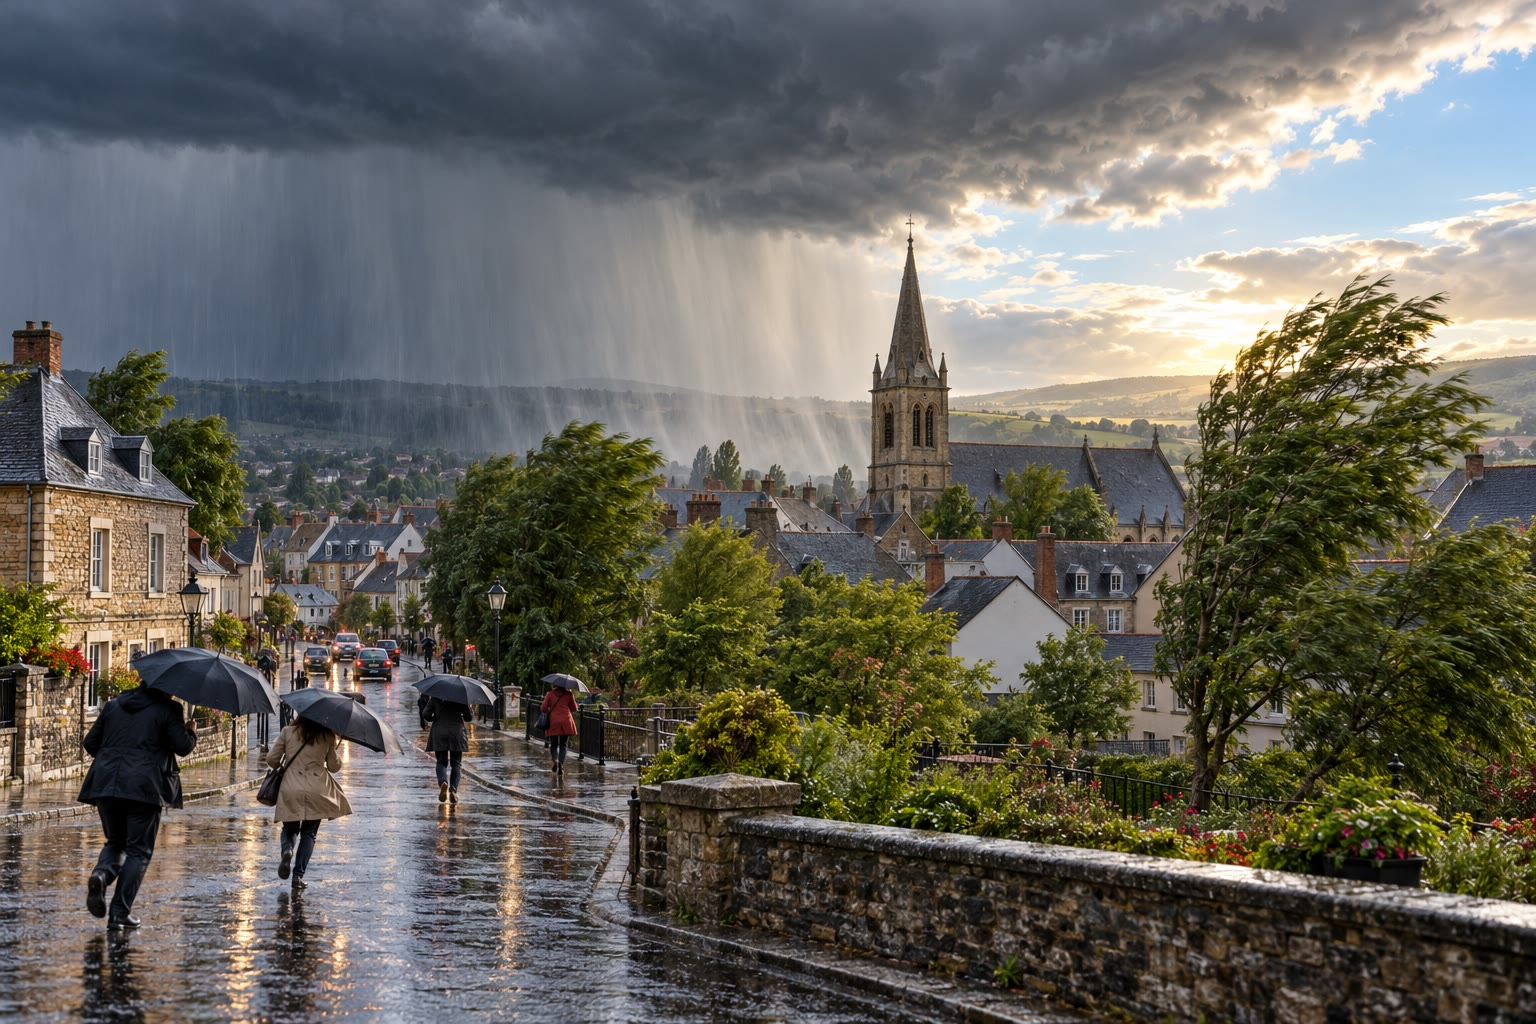
\includegraphics[width=0.6\linewidth]{images/book1/ai/g8-rain-arriving.jpg}

{\small ستار من \omterm{def:g4:clouds-rain-snow:precipitation}{المطر} يصل فوق بلدة تحت قاعدة \omterm{def:g4:clouds-rain-snow:cloud}{سحب} داكنة، بينما لا تزال
السماء صافية خلف الكنيسة (رسم توضيحي مولَّد بالذكاء الاصطناعي لمشهد
عام).}
\label{fig:g8:fronts-and-weather-maps:rain}
\end{omfigure}

رأى المتنبئون الجويون ذلك قادمًا قبل أيام. ويبين هذا الفصل كيف: فهواء
سمائنا يأتي في كتل كبيرة، والكتل تلتقي على طول جبهات، وخرائط الضغط
تبين إلى أين تتجه.

\begin{recall}
الهواء يضغط على كل ما يلامسه؛ ويقيس البارومتر هذا الضغط بالهكتوباسكال (كتب
الفيزياء)، وهو عند \omterm{def:g4:world-physical-map:altitude}{مستوى سطح البحر} نحو \qty{1013}{hPa}
(\cref{ch:g8:the-atmosphere}). وتتكون \omterm{def:g4:clouds-rain-snow:cloud}{السحب} حين يصعد هواء رطب ويبرد
(\cref{ch:g4:clouds-rain-snow}). وعند الأرض، تهب الريح من الضغط العالي نحو
الضغط المنخفض، ويحرفها دوران الأرض: إلى اليمين في \omterm{def:g3:continents-and-oceans:equator}{نصف الكرة الشمالي}.
وبين نحو \ang{30} و\ang{60}، تجلب \omterm{def:g8:winds-global-circulation:global-winds}{الرياح الغربية} \omterm{def:g5:natural-hazards:storm}{عاصفة} بعد \omterm{def:g5:natural-hazards:storm}{عاصفة}
(\cref{ch:g8:winds-global-circulation}).
\end{recall}

\section{الكتل الهوائية}

الهواء الذي يبقى أيامًا فوق المكان نفسه يكتسب طبع السطح الذي تحته. ففوق
\omterm{def:g2:water-on-earth:ocean}{محيط} دافئ يصير دافئًا رطبًا؛ وفوق يابسة متجمدة، باردًا جافًا. وحين يرحل،
يحمل هذا الطبع معه، أحيانًا آلاف الكيلومترات.
% ledger: noaa:air-mass

\begin{definition}[الكتلة الهوائية]\label{def:g8:fronts-and-weather-maps:air-mass}
\emph{الكتلة الهوائية}\index{كتلة هوائية} جسم كبير جدًا من الهواء تكاد
درجة الحرارة والرطوبة فيه تكونان متساويتين في كل مكان عند \omterm{def:g4:world-physical-map:altitude}{ارتفاع} معين. وهي
تأخذهما من المنطقة التي تكونت فيها، أي \emph{منطقة منشئها}.
\end{definition}
% ledger: noaa:air-mass

يسمي المتنبئون \omterm{def:g8:fronts-and-weather-maps:air-mass}{الكتلة الهوائية} بحرفين. الأول يقول أين تكونت: \emph{c}
(قارية) فوق اليابسة، فهي جافة؛ و\emph{m} (بحرية) فوق \omterm{def:g2:water-on-earth:ocean}{محيط}، فهي رطبة. والثاني
يقول مدى برودتها: \emph{A} (قطبية شمالية) فوق المناطق القطبية، و\emph{P}
(قطبية) فوق العروض العليا، و\emph{T} (مدارية) فوق العروض الدنيا. فهواء
\omterm{def:g5:weather-and-climate:desert}{صحراء} حارة هو cT، حار جاف؛ وهواء المنطقة القطبية الشمالية هو cA، شديد البرودة
جاف.
% ledger: noaa:air-mass

\begin{omfigure}
\begin{tikzpicture}
\begin{axis}[ommap, width=12.6cm, xmin=-100, xmax=60, ymin=10, ymax=85,
  xtick={-90,-60,...,60}, ytick={20,40,60,80},
  xticklabels={\foreignlanguage{arabic}{$90^\circ$ غ},\foreignlanguage{arabic}{$60^\circ$ غ},\foreignlanguage{arabic}{$30^\circ$ غ},$0^\circ$,\foreignlanguage{arabic}{$30^\circ$ ق},\foreignlanguage{arabic}{$60^\circ$ ق}},
  yticklabels={\foreignlanguage{arabic}{$20^\circ$ ش},\foreignlanguage{arabic}{$40^\circ$ ش},\foreignlanguage{arabic}{$60^\circ$ ش},\foreignlanguage{arabic}{$80^\circ$ ش}},
  tick label style={font=\scriptsize}]
  \addplot[fill=omLithAlluv, draw=black!45, line width=0.2pt] table {figdata/out/shared-geo-land.dat};
  \tikzset{src/.style={line width=0.9pt, fill opacity=0.35, text opacity=1, font=\scriptsize, align=center}}
  \draw[src, draw=omCold, fill=omCold!35] (axis cs:-30,79) ellipse [x radius=26, y radius=4.5];
  \node[font=\scriptsize, align=center, fill=white, inner sep=1pt] at (axis cs:-30,79) {\foreignlanguage{arabic}{\babelsublr{\textbf{cA}}: شديدة البرودة، جافة}};
  \draw[src, draw=omCold, fill=omCold!25] (axis cs:-35,55) ellipse [x radius=14, y radius=6];
  \node[font=\scriptsize, align=center, fill=white, inner sep=1pt] at (axis cs:-35,55) {\foreignlanguage{arabic}{\babelsublr{\textbf{mP}}: باردة،}\\ رطبة};
  \draw[src, draw=omCold, fill=omCold!25] (axis cs:-84,60) ellipse [x radius=12, y radius=7];
  \node[font=\scriptsize, align=center, fill=white, inner sep=1pt] at (axis cs:-84,60) {\foreignlanguage{arabic}{\babelsublr{\textbf{cP}}: باردة،}\\ جافة};
  \draw[src, draw=omCold, fill=omCold!25] (axis cs:45,62) ellipse [x radius=14, y radius=7];
  \node[font=\scriptsize, align=center, fill=white, inner sep=1pt] at (axis cs:45,62) {\foreignlanguage{arabic}{\babelsublr{\textbf{cP}}: باردة،}\\ جافة};
  \draw[src, draw=omWarm, fill=omWarm!25] (axis cs:-45,28) ellipse [x radius=16, y radius=6];
  \node[font=\scriptsize, align=center, fill=white, inner sep=1pt] at (axis cs:-45,28) {\foreignlanguage{arabic}{\babelsublr{\textbf{mT}}: دافئة،}\\ رطبة};
  \draw[src, draw=omWarm, fill=omWarm!25] (axis cs:10,24) ellipse [x radius=15, y radius=6];
  \node[font=\scriptsize, align=center, fill=white, inner sep=1pt] at (axis cs:10,24) {\foreignlanguage{arabic}{\babelsublr{\textbf{cT}}: حارة،}\\ جافة};
\end{axis}
\end{tikzpicture}

{\small مناطق منشأ نموذجية للكتل الهوائية حول شمال \omterm{def:g2:water-on-earth:ocean}{المحيط} الأطلسي (رسم
تخطيطي): فوق المنطقة القطبية الشمالية، \omterm{def:g3:continents-and-oceans:continent}{والقارات} الباردة، \omterm{def:g2:water-on-earth:ocean}{والمحيط} الشمالي،
\omterm{def:g2:water-on-earth:ocean}{والمحيط} شبه المداري، \omterm{def:g5:weather-and-climate:desert}{والصحراء} الكبرى. بالأزرق: الكتل الهوائية الباردة؛
وبالأحمر: الدافئة.}
% ledger: noaa:air-mass, data:ne-land (schematic regions)
\label{fig:g8:fronts-and-weather-maps:sources}
\end{omfigure}

\section{الجبهات}

حين تتحرك \omterm{def:g8:fronts-and-weather-maps:air-mass}{كتلة هوائية}، تلتقي بأخرى. ولا تختلط الاثنتان بسهولة: فهما تبقيان
منفصلتين، بينهما حد ضيق يتغير عنده \omterm{def:g1:watching-the-weather:weather}{الطقس}.
% ledger: mo:fronts, ucar:cold-front

\begin{definition}[الجبهة]\label{def:g8:fronts-and-weather-maps:front}
\emph{الجبهة}\index{جبهة} هي الحد عند الأرض بين كتلتين هوائيتين مختلفتين في
درجة الحرارة والرطوبة. فعند \emph{الجبهة الباردة}\index{جبهة باردة}، يندفع
هواء بارد في هواء أدفأ ويحل محله؛ وعند \emph{الجبهة الدافئة}\index{جبهة دافئة}،
يندفع هواء دافئ في هواء أبرد ويحل محله.
\end{definition}
% ledger: mo:fronts, ucar:cold-front, ucar:warm-front

الهواء البارد أكثف من الهواء الدافئ. فعند \omterm{def:g8:fronts-and-weather-maps:front}{الجبهة الباردة}، ينزلق الهواء البارد
تحت الهواء الدافئ كإسفين ويرفعه بحدة. فيصعد الهواء الدافئ الرطب بسرعة ويبني
سحبًا شاهقة، من \omterm{def:g4:clouds-rain-snow:cloud-families}{الركام} \omterm{def:g4:clouds-rain-snow:cloud-families}{والركام المزني}: فتجلب \omterm{def:g8:fronts-and-weather-maps:front}{الجبهة} زخات غزيرة، وأحيانًا بردًا
ورعدًا، وهبّات ريح وانخفاضًا مفاجئًا في درجة الحرارة. وما إن تمر حتى يتوقف
\omterm{def:g4:clouds-rain-snow:precipitation}{المطر} وتصفو السماء. \omterm{def:g8:fronts-and-weather-maps:front}{والجبهة الباردة} تتحرك بسرعة، قد تبلغ ضعف سرعة \omterm{def:g8:fronts-and-weather-maps:front}{الجبهة
الدافئة}.
% ledger: ucar:cold-front

\begin{omfigure}
\begin{tikzpicture}[font=\footnotesize, >={Stealth[length=2.2mm]}, yscale=0.7, xscale=0.95]
  % ground
  \draw[line width=0.8pt] (0,0) -- (15,0);
  % cold wedge, nose at x = 8.2
  \fill[omCold!18] (0,0) -- (0,3.4) .. controls (4.5,3.2) and (7.2,2.4) .. (7.9,0.8)
    .. controls (8.1,0.35) and (8.2,0.12) .. (8.25,0) -- cycle;
  \draw[omCold, line width=1pt] (0,3.4) .. controls (4.5,3.2) and (7.2,2.4) .. (7.9,0.8)
    .. controls (8.1,0.35) and (8.2,0.12) .. (8.25,0);
  \node[omCold, align=center] at (3.2,1.4) {\textbf{هواء بارد}\\(كثيف)};
  \node[omWarm, align=center] at (12.6,1.4) {\textbf{هواء دافئ رطب}};
  % cold air pushes
  \draw[->, omCold, line width=1.2pt] (4.6,0.5) -- (7.0,0.5);
  % warm air lifted
  \draw[->, omWarm, line width=1.2pt] (11.2,0.45) .. controls (9.4,0.6) and (8.6,1.4) .. (8.5,3.0);
  % cumulonimbus
  \fill[black!12] (7.3,2.6) .. controls (7.0,3.4) and (7.4,4.2) .. (7.9,4.5)
    .. controls (7.6,5.0) and (8.6,5.2) .. (9.4,5.1) -- (11.0,5.15)
    .. controls (10.6,4.9) and (10.2,4.8) .. (10.0,4.6)
    .. controls (10.4,4.0) and (10.2,3.0) .. (9.8,2.5) -- cycle;
  \draw[black!45] (7.3,2.6) .. controls (7.0,3.4) and (7.4,4.2) .. (7.9,4.5)
    .. controls (7.6,5.0) and (8.6,5.2) .. (9.4,5.1) -- (11.0,5.15)
    .. controls (10.6,4.9) and (10.2,4.8) .. (10.0,4.6)
    .. controls (10.4,4.0) and (10.2,3.0) .. (9.8,2.5) -- cycle;
  \node at (9.0,3.8) {ركام مزني};
  \foreach \x in {7.7,8.0,...,9.6} \draw[omCold!70, line width=0.5pt] (\x,2.45) -- (\x-0.25,0.15);
  \node[anchor=west, align=left] at (9.8,1.95) {زخات غزيرة\\وهبّات ريح};
  % motion
  \draw[->, line width=1.3pt] (5.7,4.3) -- (7.2,4.3);
  \node[anchor=east] at (5.6,4.3) {الجبهة تتقدم};
  \node[anchor=north] at (8.25,-0.1) {الجبهة عند الأرض};
  \node[anchor=north west, align=left] at (0.1,-0.1) {خلفها: أبرد، والسماء تصفو};
  \node[anchor=north east, align=right] at (15,-0.1) {أمامها: دافئ رطب};
\end{tikzpicture}

{\small \omterm{def:g8:fronts-and-weather-maps:front}{جبهة باردة} كما تُرى من الجانب (الارتفاعات مبالغ فيها كثيرًا). يندفع
الهواء البارد تحت الهواء الدافئ كإسفين؛ فيرتفع الهواء الدافئ بانحدار شديد
ويبني سحبًا شاهقة.}
% ledger: ucar:cold-front
\label{fig:g8:fronts-and-weather-maps:cold}
\end{omfigure}

عند \omterm{def:g8:fronts-and-weather-maps:front}{الجبهة الدافئة}، لا يستطيع الهواء الدافئ الخفيف أن يزيح الهواء البارد عن
الأرض: فهو يتسلقه ببطء، على منحدر طويل لطيف. ولذلك تظهر سحبه بعيدًا جدًا
أمام \omterm{def:g8:fronts-and-weather-maps:front}{الجبهة}، عاليًا في السماء: أولًا خطوط رقيقة من \omterm{def:g4:clouds-rain-snow:cloud-families}{السمحاق}، ثم حجاب من
\omterm{def:g4:clouds-rain-snow:cloud-families}{السمحاق} \omterm{def:g4:clouds-rain-snow:cloud-families}{الطبقي}، ثم \omterm{def:g4:clouds-rain-snow:cloud-families}{الطبقي} المتوسط الرمادي. وكلما اقتربت \omterm{def:g8:fronts-and-weather-maps:front}{الجبهة}، انخفضت
\omterm{def:g4:clouds-rain-snow:cloud}{السحب} وازدادت سماكة وبدأ \omterm{def:g4:clouds-rain-snow:precipitation}{مطر} طويل متواصل. وبعد أن تمر، يصير الهواء أدفأ
وأرطب.
% ledger: ucar:warm-front, bom:isobars (warm front: steady rain, grey skies)

\begin{omfigure}
\begin{tikzpicture}[font=\footnotesize, >={Stealth[length=2.2mm]}]
  \draw[line width=0.8pt] (0,0) -- (15,0);
  % cold air ahead (right), warm air climbing a gentle slope from the front at x = 2.2
  \fill[omCold!18] (2.2,0) .. controls (6,0.9) and (10,2.2) .. (15,3.4) -- (15,0) -- cycle;
  \draw[omCold, line width=1pt] (2.2,0) .. controls (6,0.9) and (10,2.2) .. (15,3.4);
  \node[omCold, align=center] at (11.8,0.75) {\textbf{هواء بارد}};
  \node[omWarm, align=center] at (1.4,1.6) {\textbf{هواء}\\\textbf{دافئ رطب}};
  \draw[->, omWarm, line width=1.2pt] (1.0,0.45) .. controls (4.5,0.9) and (8.5,2.4) .. (12.4,3.4);
  % clouds: nimbostratus near the front, altostratus, cirrostratus, cirrus far ahead
  \fill[black!18] (2.4,0.7) .. controls (3.2,1.8) and (5.5,2.3) .. (6.6,2.4) -- (6.4,1.25) .. controls (5,1.0) and (3.8,0.7) .. cycle;
  \node at (5.4,1.62) {المزن الطبقي};
  \foreach \x in {3.0,3.3,...,5.7} \draw[omCold!70, line width=0.5pt] (\x,0.95) -- (\x-0.2,0.25);
  \fill[black!10, rounded corners=4pt] (6.4,2.65) rectangle (10.0,3.25);
  \node at (8.2,2.95) {الطبقي المتوسط};
  \fill[black!6, rounded corners=4pt] (9.6,3.75) rectangle (12.6,4.15);
  \node at (11.1,3.95) {السمحاق الطبقي};
  \foreach \x in {12.6,13.2,13.8} \draw[black!35, line width=0.6pt] (\x,4.55) .. controls (\x+0.2,4.75) and (\x+0.4,4.6) .. (\x+0.55,4.85);
  \node[anchor=south] at (13.4,4.9) {السمحاق};
  \draw[->, line width=1.3pt] (2.6,4.3) -- (4.1,4.3);
  \node[anchor=east] at (2.5,4.3) {الجبهة تتقدم};
  \node[anchor=north] at (2.2,-0.1) {الجبهة عند الأرض};
  \node[anchor=north east] at (15,-0.1) {بعيدًا في الأمام: أولى السحب العالية};
\end{tikzpicture}

{\small \omterm{def:g8:fronts-and-weather-maps:front}{جبهة دافئة} كما تُرى من الجانب (الارتفاعات مبالغ فيها كثيرًا). يتسلق
الهواء الدافئ الهواء البارد ببطء؛ وتنخفض سحبه وتزداد سماكة كلما اقتربت
\omterm{def:g8:fronts-and-weather-maps:front}{الجبهة}، \omterm{def:g4:clouds-rain-snow:precipitation}{والمطر} طويل متواصل.}
% ledger: ucar:warm-front
\label{fig:g8:fronts-and-weather-maps:warm}
\end{omfigure}

على \omterm{def:g2:drawing-to-map:map}{خريطة} \omterm{def:g1:watching-the-weather:weather}{الطقس}، تُرسم \omterm{def:g8:fronts-and-weather-maps:front}{الجبهة الباردة} خطًا أزرق عليه مثلثات، \omterm{def:g8:fronts-and-weather-maps:front}{والجبهة الدافئة}
خطًا أحمر عليه أنصاف دوائر. وتقع الرموز على الجانب الذي تتحرك نحوه \omterm{def:g8:fronts-and-weather-maps:front}{الجبهة}.
وحين تلحق \omterm{def:g8:fronts-and-weather-maps:front}{جبهة باردة} سريعة \omterm{def:g8:fronts-and-weather-maps:front}{بجبهة دافئة}، تتحدان في \emph{\omterm{def:g8:fronts-and-weather-maps:front}{جبهة} مسدودة}،
تُرسم بالبنفسجي وعليها الرمزان كلاهما.
% ledger: mo:fronts, ucar:cold-front

\section{المنخفضات والمرتفعات الجوية}

تولد الجبهات في دوامات الهواء الكبرى التي تعبر العروض الوسطى. فحيث يصعد
الهواء، يكون الضغط عند الأرض أدنى منه في كل ما حوله؛ وحيث يهبط، يكون الضغط
أعلى.
% ledger: bom:highs-lows

\begin{definition}[المنخفض الجوي والمرتفع الجوي]\label{def:g8:fronts-and-weather-maps:depression}
\emph{المنخفض الجوي}\index{منخفض جوي} منطقة يكون فيها الضغط عند \omterm{def:g4:world-physical-map:altitude}{مستوى
سطح البحر} أدنى منه في كل ما حولها. و\emph{المرتفع الجوي}\index{مرتفع جوي}
منطقة يكون فيها الضغط أعلى منه في كل ما حولها.
\end{definition}
% ledger: bom:isobars, bom:highs-lows
\phantomsection\label{def:g8:fronts-and-weather-maps:anticyclone}

تهب الريح من المرتفع نحو المنخفض، لكن دوران الأرض يحرفها، فتنتهي إلى أن
تهب حول المراكز تقريبًا. ففي \omterm{def:g3:continents-and-oceans:equator}{نصف الكرة الشمالي} تدور عكس اتجاه عقارب الساعة
حول \omterm{def:g8:fronts-and-weather-maps:depression}{المنخفض الجوي} ومع اتجاه عقارب الساعة حول \omterm{def:g8:fronts-and-weather-maps:depression}{المرتفع الجوي}؛ وفي \omterm{def:g3:continents-and-oceans:equator}{نصف الكرة
الجنوبي}، العكس. وفي \omterm{def:g8:fronts-and-weather-maps:depression}{المنخفض الجوي}، يتدفق الهواء إلى الداخل قرب الأرض، ويصعد
ويبرد ويكوّن \omterm{def:g4:clouds-rain-snow:cloud}{السحب}: فالمنخفضات الجوية تجلب \omterm{def:g4:clouds-rain-snow:cloud}{السحب} \omterm{def:g4:clouds-rain-snow:precipitation}{والمطر} والريح، وجبهاتها.
وفي \omterm{def:g8:fronts-and-weather-maps:depression}{المرتفع الجوي}، يهبط الهواء ويسخن وهو ينزل: فالمرتفعات الجوية تجلب طقسًا
جافًا مستقرًا ورياحًا خفيفة. ويبلغ الضغط في مركز \omterm{def:g8:fronts-and-weather-maps:depression}{المرتفع الجوي} النموذجي نحو
\qty{1020}{hPa} أو أكثر؛ أما \omterm{def:g8:fronts-and-weather-maps:depression}{المنخفض الجوي} العميق فينزل ضغطه إلى أقل من
\qty{980}{hPa}.
% ledger: bom:highs-lows, bom:isobars, mo:global-circ

\begin{omfigure}
\begin{minipage}[c]{0.36\linewidth}\centering
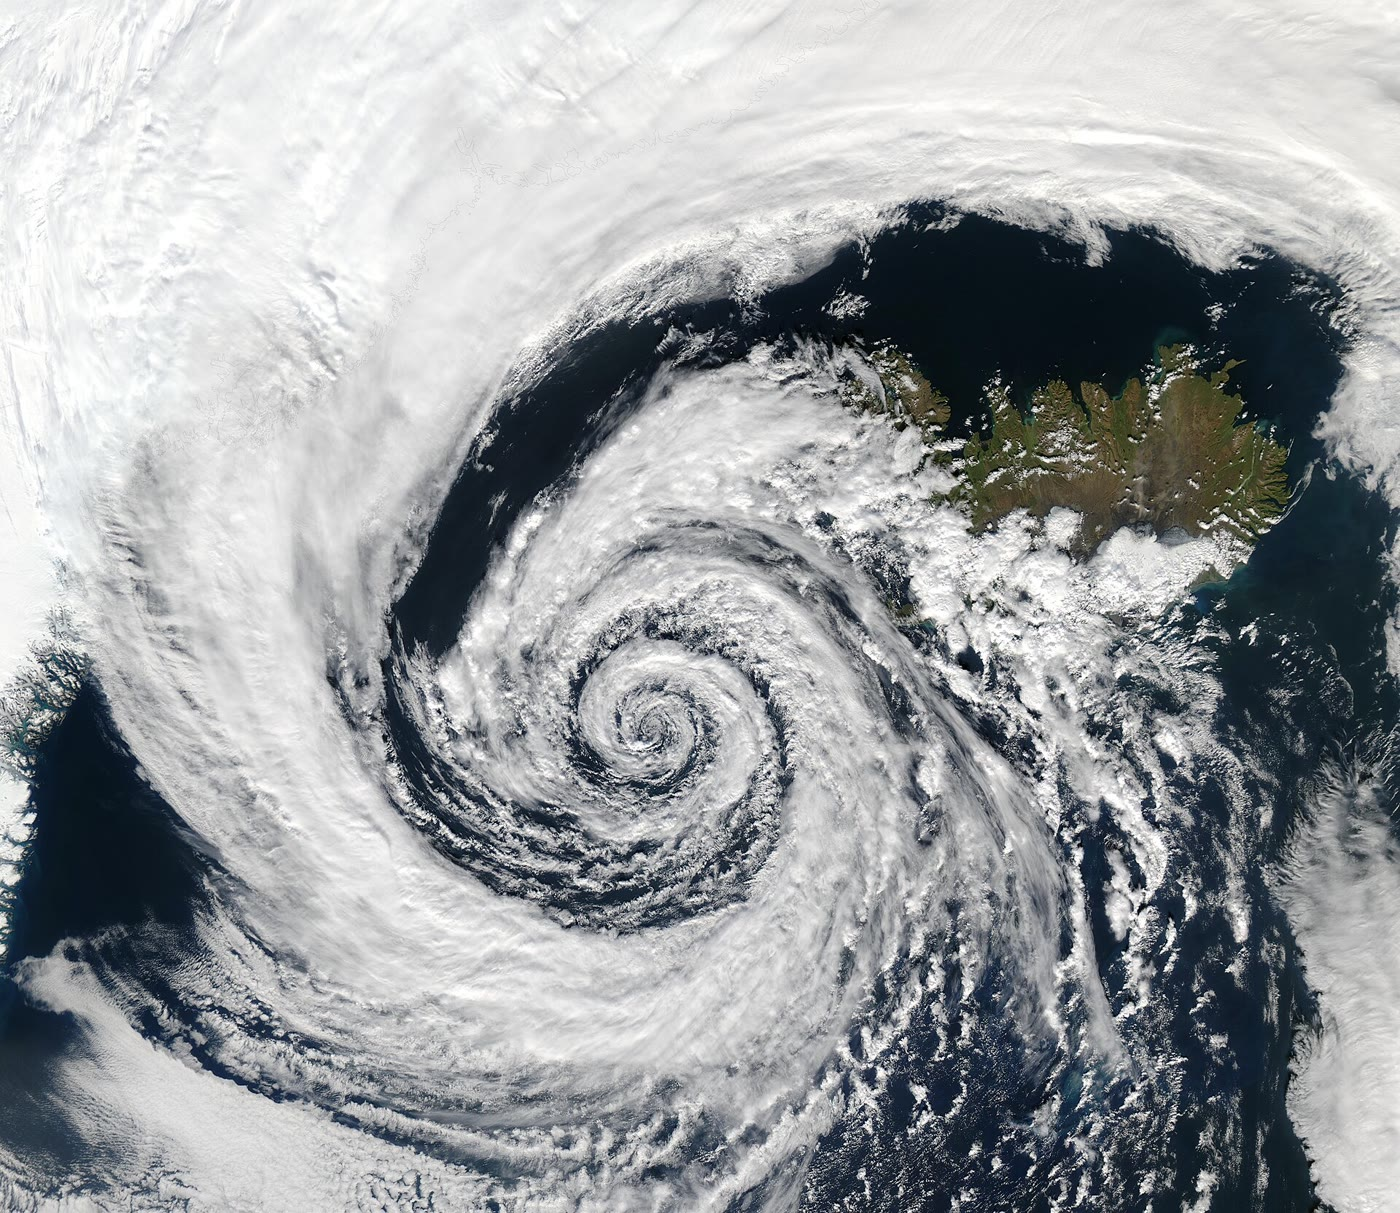
\includegraphics[width=\linewidth]{images/book1/g8-iceland-low.jpg}
\end{minipage}\hfill
\begin{minipage}[c]{0.6\linewidth}\raggedright
{\small \omterm{def:g8:fronts-and-weather-maps:depression}{منخفض جوي} جنوب غرب آيسلندا (الجزيرة التي في أعلى اليمين) كما رآه
القمر الصناعي أكوا التابع لوكالة ناسا في 4~سبتمبر 2003. تلتف سحبه حلزونيًا نحو
المركز، دائرة عكس اتجاه عقارب الساعة كما في كل \omterm{def:g8:fronts-and-weather-maps:depression}{منخفض جوي} في \omterm{def:g3:continents-and-oceans:equator}{نصف الكرة
الشمالي}. ناسا، مركز غودارد لرحلات الفضاء، فريق الاستجابة السريعة لجهاز
موديس، جاك ديكلوتر (ملك عام، عبر ويكيميديا كومنز).}
\end{minipage}
% ledger: commons:iceland-low, bom:highs-lows
\label{fig:g8:fronts-and-weather-maps:iceland}
\end{omfigure}

\section{خطوط تساوي الضغط وخرائط الطقس}

لرؤية المنخفضات والمرتفعات الجوية، يرسم المتنبئون خرائط للضغط. فكل محطة
تقيس ضغطها وتردّه إلى \omterm{def:g4:world-physical-map:altitude}{مستوى سطح البحر}، كي يمكن مقارنة محطة على \omterm{def:g1:landscapes-around-us:landform}{جبل} بمحطة
على \omterm{def:g1:landscapes-around-us:water}{الساحل}. ثم تُرسم خطوط تمر بكل الأماكن التي يتساوى فيها
الضغط.
% ledger: bom:isobars

\begin{definition}[خط تساوي الضغط]\label{def:g8:fronts-and-weather-maps:isobar}
\emph{خط تساوي الضغط}\index{خط تساوي الضغط} خط على \omterm{def:g2:drawing-to-map:map}{الخريطة} يصل بين أماكن
يتساوى فيها الضغط عند \omterm{def:g4:world-physical-map:altitude}{مستوى سطح البحر}. وتُكتب عليه قيمته بالهكتوباسكال،
وكثيرًا ما تُرسم هذه الخطوط كل \qty{4}{hPa}.
\end{definition}
% ledger: bom:isobars (the 4 hPa step is the one of this book's maps)

حول \omterm{def:g8:fronts-and-weather-maps:depression}{المنخفض الجوي} تشكّل \omterm{def:g8:fronts-and-weather-maps:isobar}{خطوط تساوي الضغط} حلقات مغلقة، أدنى ضغط فيها في
المركز، ويُرمز إليه بالحرف م؛ وحول \omterm{def:g8:fronts-and-weather-maps:depression}{المرتفع الجوي} تشكّل حلقات أعلى ضغط فيها
في المركز، ويُرمز إليه بالحرف ع. وحيث تتقارب \omterm{def:g8:fronts-and-weather-maps:isobar}{خطوط تساوي الضغط}، يتغير الضغط
بسرعة من مكان إلى الذي يليه، وتكون الريح قوية؛ وحيث تتباعد، تكون الريح
خفيفة.
% ledger: bom:isobars

\begin{omfigure}
\begin{tikzpicture}
\begin{axis}[width=14cm, axis equal image, xmin=0, xmax=2400, ymin=0, ymax=1600,
  hide axis, clip=true, axis background/.style={fill=white}]
  \addplot[isobar] table {figdata/out/grade-8-weather_map-isobars.dat};
  \addplot[warm front] table {figdata/out/grade-8-weather_map-warm.dat};
  \addplot[cold front] table {figdata/out/grade-8-weather_map-cold.dat};
  \addplot[quiver={u=\thisrow{u}, v=\thisrow{v}}, -{Stealth[length=1.5mm]}, omMeth, line width=0.6pt]
    table[x=x, y=y] {figdata/out/grade-8-weather_map-winds.dat};
  \addplot[only marks, mark=none, nodes near coords, point meta=explicit symbolic,
    every node near coord/.style={anchor=center, font=\tiny, fill=white, inner sep=0.6pt}]
    table[x=x, y=y, meta=level] {figdata/out/grade-8-weather_map-labels.dat};
  \node[font=\Large\bfseries, omCold, fill=white, inner sep=1pt] at (axis cs:690,1010) {م};
  \node[font=\scriptsize, anchor=north, fill=white, inner sep=0.5pt] at (axis cs:690,968) {980};
  \node[font=\Large\bfseries, omWarm] at (axis cs:1950,520) {ع};
  \node[font=\scriptsize, anchor=north] at (axis cs:1950,485) {1034};
  \addplot[only marks, mark=square*, mark size=2pt, black] table[x=x, y=y] {figdata/out/grade-8-weather_map-town.dat};
  \node[font=\footnotesize\bfseries, anchor=west, fill=white, inner sep=1pt] at (axis cs:870,380) {T};
  \fill[white] (axis cs:1930,1450) rectangle (axis cs:2290,1585);
  \draw[line width=1pt] (axis cs:1950,1480) -- (axis cs:2250,1480);
  \pgfplotsinvokeforeach{1950,2050,2150,2250}{\draw (axis cs:#1,1460) -- (axis cs:#1,1500);}
  \node[font=\scriptsize, anchor=south] at (axis cs:2100,1495) {\babelsublr{300 km}};
\end{axis}
\end{tikzpicture}

{\small \omterm{def:g2:drawing-to-map:map}{خريطة} \omterm{def:g1:watching-the-weather:weather}{طقس} ليوم متخيَّل في \omterm{def:g3:continents-and-oceans:equator}{نصف الكرة الشمالي}، محسوبة من نموذج
للضغط. \omterm{def:g8:fronts-and-weather-maps:isobar}{خطوط تساوي الضغط} كل \qty{4}{hPa}؛ \omterm{def:g8:fronts-and-weather-maps:depression}{والمنخفض الجوي} م (\qty{980}{hPa})
يحمل \omterm{def:g8:fronts-and-weather-maps:front}{جبهة دافئة} (بالأحمر) \omterm{def:g8:fronts-and-weather-maps:front}{وجبهة باردة} (بالأزرق)؛ \omterm{def:g8:fronts-and-weather-maps:depression}{والمرتفع الجوي} ع
(\qty{1034}{hPa}) يقع إلى الشرق. الأسهم الخضراء: الريح، وهي أطول حيث تكون
أقوى. T: بلدة المسألة.}
% ledger: bom:isobars, bom:highs-lows, mo:fronts (figdata/grade-8/weather_map.py)
\label{fig:g8:fronts-and-weather-maps:map}
\end{omfigure}

\begin{method}[قراءة خريطة الطقس]
\begin{enumerate}
  \item جد المراكز: م للمنخفضات الجوية، وع للمرتفعات الجوية،
        مع ضغوطها.
  \item اقرأ \omterm{def:g8:fronts-and-weather-maps:isobar}{خطوط تساوي الضغط}: فقيمها ترتفع نحو ع وتنخفض نحو م.
        والخطوط المتقاربة تعني ريحًا قوية.
  \item جد اتجاه الريح: ففي \omterm{def:g3:continents-and-oceans:equator}{نصف الكرة الشمالي} تهب على طول \omterm{def:g8:fronts-and-weather-maps:isobar}{خطوط تساوي الضغط}
        تقريبًا، والضغط المنخفض على يسارها، منحرفة قليلًا نحو المنخفض.
  \item جد الجبهات واتجاه حركتها (جانب رموزها)، ثم الهواء على كل
        جانب: ما الذي سيأتي بعد ذلك؟
\end{enumerate}
\end{method}
% ledger: bom:isobars, bom:highs-lows, mo:fronts

\begin{example}[الطقس في البلدة T]
على \omterm{def:g2:drawing-to-map:map}{الخريطة}، تقع T جنوب \omterm{def:g8:fronts-and-weather-maps:front}{الجبهة الدافئة} وشرق \omterm{def:g8:fronts-and-weather-maps:front}{الجبهة الباردة}: في الهواء
الدافئ بين الجبهتين. \omterm{def:g8:fronts-and-weather-maps:front}{فالجبهة الدافئة} قد مرت بها. \omterm{def:g8:fronts-and-weather-maps:isobar}{وخطوط تساوي الضغط} تمتد هناك
من الجنوب الغربي إلى الشمال الشرقي، والمنخفض إلى الشمال الغربي: فالريح تهب
من الجنوب الغربي، دافئة رطبة. \omterm{def:g8:fronts-and-weather-maps:front}{والجبهة الباردة} قادمة من الغرب. ومثلثاتها تشير
إلى الشرق، نحو البلدة: ففي غضون ساعات ستأتي فترة قصيرة من الزخات الغزيرة
والهبّات، ثم تتحول الريح إلى غربية أو شمالية غربية، ويبرد الهواء وتصفو
السماء.
\end{example}
% ledger: ucar:cold-front (figdata/grade-8/weather_map.py: wind at T from 227 degrees)

البارومتر يعطي إنذاره الخاص، حتى دون \omterm{def:g2:drawing-to-map:map}{خريطة}. افترض أن \omterm{def:g2:drawing-to-map:map}{الخريطة} أعلاه كلها انجرفت
شرقًا، دون أن تتغير، بسرعة \qty{40}{km} في الساعة، وأن بارومترًا مسجّلًا كان
في محطة S، شرق الجبهات. فعلى مدى يومين ونصف كان سيرسم التسجيل
الذي أدناه.

\begin{omfigure}
\begin{tikzpicture}
\begin{axis}[width=0.86\linewidth, height=5.4cm, xmin=0, xmax=60, ymin=980, ymax=1040,
  xtick={0,12,...,60}, ytick={980,990,...,1040},
  xlabel={\foreignlanguage{arabic}{الساعات منذ بداية التسجيل}}, ylabel={\foreignlanguage{arabic}{الضغط \babelsublr{(hPa)}}},
  axis x line=bottom, axis y line=left, axis line style={-},
  grid=major, grid style={black!10},
  tick label style={font=\scriptsize}, label style={font=\small}, clip=false]
  \draw[omWarm!80!black, dashed] (axis cs:26.28,980) -- (axis cs:26.28,1040);
  \draw[omCold!80!black, dashed] (axis cs:38.49,980) -- (axis cs:38.49,1040);
  \node[font=\scriptsize, omWarm!80!black, anchor=south, fill=white, inner sep=1pt] at (axis cs:26.28,1032) {جبهة دافئة};
  \node[font=\scriptsize, omCold!80!black, anchor=south, fill=white, inner sep=1pt] at (axis cs:38.49,1032) {جبهة باردة};
  \addplot[black!80, line width=1pt] table[x=hour, y=p_hPa] {figdata/out/grade-8-barogram-trace.dat};
  \node[font=\scriptsize, anchor=north west, align=left] at (axis cs:2,1028) {مرتفع جوي\\طقس مستقر};
  \node[font=\scriptsize, anchor=west] at (axis cs:39.5,986) {الأدنى};
\end{axis}
\end{tikzpicture}

{\small تسجيل بارومتر في المحطة S بينما تنجرف \omterm{def:g2:drawing-to-map:map}{الخريطة} أعلاه شرقًا بسرعة
\qty{40}{km} في الساعة (حالة متخيَّلة، محسوبة من حقل الضغط في \omterm{def:g2:drawing-to-map:map}{الخريطة}).
الخطان المتقطعان: مرور \omterm{def:g8:fronts-and-weather-maps:front}{الجبهة الدافئة} \omterm{def:g8:fronts-and-weather-maps:front}{والجبهة الباردة}
بالمحطة.}
% ledger: (invented region: weather situation of figdata/grade-8/weather_map.py, record from figdata/grade-8/barogram.py)
\end{omfigure}

\begin{example}[قراءة تسجيل البارومتر]\label{ex:g8:fronts-and-weather-maps:barogram}
في الساعات الثماني الأولى يرتفع الضغط إلى نحو \qty{1031}{hPa}: \omterm{def:g8:fronts-and-weather-maps:depression}{فالمرتفع
الجوي} يمر فوق S، \omterm{def:g1:watching-the-weather:weather}{والطقس} مستقر. ثم ينخفض طوال 30
ساعة، بنحو \qty{45}{hPa}: \omterm{def:g8:fronts-and-weather-maps:depression}{فالمنخفض الجوي} قادم. ويكون انخفاضه أسرع ما يكون قبل
مرور \omterm{def:g8:fronts-and-weather-maps:front}{الجبهة الدافئة} ببضع ساعات، وأبطأ في الهواء الدافئ الذي خلفها،
ويبلغ أدناه، نحو \qty{986}{hPa}، لحظة مرور \omterm{def:g8:fronts-and-weather-maps:front}{الجبهة الباردة} تمامًا. ثم يرتفع:
\omterm{def:g8:fronts-and-weather-maps:depression}{فالمنخفض الجوي} يبتعد، والهواء الأبرد والأصفى الذي خلف \omterm{def:g8:fronts-and-weather-maps:front}{الجبهة الباردة}
يصل.
% ledger: (invented region: figdata/grade-8/barogram.py), bom:highs-lows
\end{example}

\section{كيف يُصنع التنبؤ بالطقس}

\begin{definition}[التنبؤ بالطقس]\label{def:g8:fronts-and-weather-maps:forecast}
\emph{التنبؤ بالطقس}\index{تنبؤ بالطقس} بيان \omterm{def:g1:watching-the-weather:weather}{للطقس} المتوقع في مكان ما خلال
الساعات أو الأيام القادمة، يُستخلص من أرصاد الغلاف الجوي ومن قوانين
الفيزياء.
\end{definition}
% ledger: mo:how-forecasts

يُصنع \omterm{def:g8:fronts-and-weather-maps:forecast}{التنبؤ بالطقس} في ثلاث خطوات. أولًا، تجري هيئات الأرصاد في أنحاء العالم
ملايين الأرصاد كل يوم: درجة الحرارة، \omterm{def:g4:clouds-rain-snow:precipitation}{والهطول}، والضغط، والريح والرطوبة،
تُقاس في محطات أرضية، وفي \omterm{def:g2:water-on-earth:ocean}{البحر}، وبوساطة بالونات الأرصاد، والرادار، ومن
الأقمار الصناعية. ثم تُدخل هذه الأرصاد في نماذج حاسوبية: فتحسب حواسيب
فائقة القدرة، خطوة بعد خطوة، كيف سيتغير الغلاف الجوي انطلاقًا من حالته
الراهنة. وأخيرًا، يقرأ المتنبئون النتائج، ويقارنونها بما يعرفونه عن
منطقتهم، ويكتبون التنبؤ.
% ledger: mo:how-forecasts

\begin{history}[أول تنبؤ جوي للعموم]
في عام 1854 عُيّن ضابط بحري، هو روبرت فيتزروي، على رأس مكتب جديد للأرصاد في
لندن. وكل صباح في الساعة~9، كانت محطات على طول \omterm{def:g1:landscapes-around-us:water}{السواحل} تقيس \omterm{def:g1:watching-the-weather:weather}{الطقس} وترسل
قراءاتها إلى لندن بالتلغراف، أحدث اختراعات ذلك الزمن. وفي عام 1859 أغرقت
\omterm{def:g5:natural-hazards:storm}{عاصفة} رهيبة، هي \omterm{def:g5:natural-hazards:storm}{عاصفة} \emph{رويال تشارتر}، سفنًا كثيرة؛ فأنشأ فيتزروي عندئذ
خدمة لإنذار البحارة بالعواصف، بدأت في فبراير 1861. وفي
1~أغسطس 1861 ذهب أبعد من ذلك ونشر أول تنبؤ جوي للعموم في صحيفة،
هي \emph{التايمز}. وكانت تنبؤاته تنظر إلى ما بعد يوم أو يومين
وكانت عامة جدًا؛ لكنها كانت بداية التنبؤات التي نقرؤها اليوم.
\end{history}
% ledger: mo:fitzroy

لقد صارت التنبؤات أفضل بكثير. فعلى مدى العقود الماضية، كسب المتنبئون نحو يوم
إضافي من التنبؤ الجيد كل عشر سنوات: فالتنبؤ لأربعة أيام مقبلة صار اليوم بجودة
التنبؤ ليوم واحد قبل ثلاثين سنة. لكن كلما نظر التنبؤ أبعد، قل يقينه، لأن
الأخطاء الصغيرة في الأرصاد الابتدائية تكبر كلما تقدم الحاسوب في
الزمن.
% ledger: bauer:day-per-decade, mo:accuracy

\begin{inthefield}[مراقبة وصول جبهة]
في يوم يعلن فيه التنبؤ عن \omterm{def:g8:fronts-and-weather-maps:front}{جبهة}، انظر إلى السماء كل بضع ساعات ودوّن الوقت،
\omterm{def:g4:clouds-rain-snow:cloud}{والسحب}، والريح ودرجة الحرارة. فقبل \omterm{def:g8:fronts-and-weather-maps:front}{الجبهة الدافئة}، هل تأتي خطوط \omterm{def:g4:clouds-rain-snow:cloud-families}{السمحاق}
العالية أولًا؟ وحين تمر \omterm{def:g8:fronts-and-weather-maps:front}{جبهة باردة}، هل تنخفض درجة الحرارة وتتغير الريح؟ ثم
قارن ملاحظاتك \omterm{def:g2:drawing-to-map:map}{بخريطة} \omterm{def:g1:watching-the-weather:weather}{الطقس} لذلك اليوم.
\end{inthefield}

\section{تمارين}

\begin{exercise}[$\star$]\label{exo:g8:fronts-and-weather-maps:1}
أعطِ معنى كل زوج من الحروف وقل هل \omterm{def:g8:fronts-and-weather-maps:air-mass}{الكتلة الهوائية} دافئة أم باردة، رطبة أم
جافة: (أ) mT؛ (ب) cP؛ (ج) cT؛ (د) mP.
\end{exercise}

\begin{exercise}[$\star$]\label{exo:g8:fronts-and-weather-maps:2}
صِل كل علامة من علامات \omterm{def:g2:drawing-to-map:map}{خريطة} \omterm{def:g1:watching-the-weather:weather}{الطقس} بمعناها: خط أزرق عليه مثلثات؛ خط أحمر
عليه أنصاف دوائر؛ خط يصل بين أماكن متساوية الضغط؛ الحرف ع؛ الحرف
م.
\end{exercise}

\begin{exercise}[$\star$]\label{exo:g8:fronts-and-weather-maps:3}
صواب أم خطأ؟ صحّح الجمل الخاطئة. (أ) تجلب المرتفعات الجوية عادة طقسًا
مستقرًا. (ب) تصل \omterm{def:g4:clouds-rain-snow:cloud}{سحب} \omterm{def:g8:fronts-and-weather-maps:front}{الجبهة الدافئة} بعد \omterm{def:g8:fronts-and-weather-maps:front}{الجبهة}. (ج) \omterm{def:g8:fronts-and-weather-maps:isobar}{خطوط تساوي الضغط}
المتقاربة تعني ريحًا خفيفة. (د) الهواء البارد أكثف من الهواء
الدافئ.
\end{exercise}

\begin{exercise}[$\star$]\label{exo:g8:fronts-and-weather-maps:4}
على \omterm{def:g2:drawing-to-map:map}{خريطة} \omterm{def:g1:watching-the-weather:weather}{الطقس} في هذا الفصل: (أ) ما الضغط في مركز \omterm{def:g8:fronts-and-weather-maps:depression}{المنخفض الجوي}؟ (ب) وفي
مركز \omterm{def:g8:fronts-and-weather-maps:depression}{المرتفع الجوي}؟ (ج) كم هكتوباسكالًا تفصل بين خطين متجاورين من \omterm{def:g8:fronts-and-weather-maps:isobar}{خطوط
تساوي الضغط}؟ (د) بكم هكتوباسكالًا يختلف الضغط بين
المركزين؟
\end{exercise}

\begin{exercise}[$\star\star$]\label{exo:g8:fronts-and-weather-maps:5}
رتّب هذه الأحداث بالترتيب الذي تقع به حين تقترب \omterm{def:g8:fronts-and-weather-maps:front}{جبهة دافئة} وتمر: \omterm{def:g4:clouds-rain-snow:precipitation}{مطر}
متواصل؛ خطوط رقيقة من \omterm{def:g4:clouds-rain-snow:cloud-families}{السمحاق}؛ حجاب رمادي من \omterm{def:g4:clouds-rain-snow:cloud-families}{الطبقي} المتوسط؛ هواء أدفأ
وأرطب؛ \omterm{def:g4:clouds-rain-snow:cloud}{السحب} تنخفض وتزداد سماكة.
\end{exercise}

\begin{exercise}[$\star\star$]\label{exo:g8:fronts-and-weather-maps:6}
اشرح لماذا تكون \omterm{def:g4:clouds-rain-snow:cloud}{سحب} \omterm{def:g8:fronts-and-weather-maps:front}{الجبهة الباردة} شاهقة، بينما تنتشر \omterm{def:g4:clouds-rain-snow:cloud}{سحب} \omterm{def:g8:fronts-and-weather-maps:front}{الجبهة الدافئة} في
طبقات. استعمل الكلمات \emph{إسفين}،
\emph{شديد الانحدار}، \emph{منحدر لطيف}.
\end{exercise}

\begin{exercise}[$\star\star$]\label{exo:g8:fronts-and-weather-maps:7}
على \omterm{def:g2:drawing-to-map:map}{خريطة} \omterm{def:g1:watching-the-weather:weather}{الطقس}: (أ) أين تكون الريح أقوى، قرب م أم قرب ع؟
كيف تعرف ذلك؟ (ب) شمال م، من أي اتجاه تهب الريح؟
(ج) وجنوب ع؟ (د) هل تدور الريح مع اتجاه عقارب الساعة أم عكسه
حول م؟
\end{exercise}

\begin{exercise}[$\star\star$]\label{exo:g8:fronts-and-weather-maps:8}
يقرأ بارومتر في بلدة \qty{1016}{hPa} في الساعة \babelsublr{6:00}، و\qty{1009}{hPa} في الساعة
\babelsublr{12:00} و\qty{1003}{hPa} في الساعة \babelsublr{18:00}. (أ) بكم ينخفض الضغط
في 12 ساعة؟ (ب) ما القادم نحو البلدة، \omterm{def:g8:fronts-and-weather-maps:depression}{منخفض جوي} أم
\omterm{def:g8:fronts-and-weather-maps:depression}{مرتفع جوي}؟ (ج) ما \omterm{def:g1:watching-the-weather:weather}{الطقس} الذي يمكن أن تتوقعه البلدة؟
\end{exercise}

\begin{exercise}[$\star\star$]\label{exo:g8:fronts-and-weather-maps:9}
هواء بقي أسبوعًا فوق \omterm{def:g5:weather-and-climate:desert}{الصحراء} الكبرى يتحرك شمالًا فوق \omterm{def:g2:water-on-earth:ocean}{البحر} الأبيض
المتوسط. (أ) سمِّ هذه \omterm{def:g8:fronts-and-weather-maps:air-mass}{الكتلة الهوائية} بحرفيها. (ب) هل هي
حارة أم باردة، رطبة أم جافة، حين ترحل؟ (ج) ما الذي قد يتغير في
طبعها وهي تعبر \omterm{def:g2:water-on-earth:ocean}{البحر}؟
\end{exercise}

\begin{exercise}[$\star\star$]\label{exo:g8:fronts-and-weather-maps:10}
التنبؤ لأربعة أيام مقبلة صار اليوم بجودة التنبؤ ليوم واحد قبل ثلاثين
سنة. (أ) كم يومًا من التنبؤ الجيد كُسبت في ثلاثين سنة؟ (ب) كم يكون ذلك
لكل عشر سنوات؟ (ج) لو استمر التقدم نفسه، فبعد كم سنة يصير التنبؤ لخمسة أيام
بجودة التنبؤ ليوم واحد اليوم؟
\end{exercise}

\begin{exercise}[$\star\star\star$]\label{exo:g8:fronts-and-weather-maps:11}
على \omterm{def:g2:drawing-to-map:map}{خريطة} \omterm{def:g1:watching-the-weather:weather}{الطقس}، استعمل \omterm{def:g2:drawing-to-map:scale}{مقياس الرسم}. (أ) كم كيلومترًا تقريبًا تفصل بين
المركز م والمركز ع؟ (ب) قرب م، يتباعد خطان متجاوران من \omterm{def:g8:fronts-and-weather-maps:isobar}{خطوط تساوي الضغط} نحو
\qty{80}{km}. فبكم هكتوباسكالًا يتغير الضغط على مسافة \qty{100}{km} هناك؟ (ج) قرب ع، يتباعد خطان
متجاوران نحو \qty{140}{km}. السؤال نفسه. (د) أين تكون
الريح أقوى؟ وهل تتفق أسهم \omterm{def:g2:drawing-to-map:map}{الخريطة} مع ذلك؟
\end{exercise}

\begin{exercise}[$\star\star\star$]\label{exo:g8:fronts-and-weather-maps:12}
تقع \omterm{def:g8:fronts-and-weather-maps:front}{جبهة باردة} على بعد \qty{300}{km} غرب بلدة وتتحرك شرقًا بسرعة
\qty{50}{km} في الساعة؛ وتقع \omterm{def:g8:fronts-and-weather-maps:front}{جبهة دافئة} على بعد \qty{200}{km} غرب بلدة
أخرى وتتحرك بنصف تلك السرعة. (أ) أي الجبهتين تبلغ بلدتها
أولًا، وقبل الأخرى بكم ساعة؟ (ب) صف \omterm{def:g1:watching-the-weather:weather}{الطقس} الذي ستراه كل بلدة
حين تمر جبهتها. (ج) أي البلدتين ستكون أدفأ بعد أن تمر
جبهتها؟
\end{exercise}

\section{مسألة: هل ستُلغى المباراة بسبب المطر؟}

\begin{problem}[{مسألة نهاية الأسبوع --- مباراة كرة قدم مقررة في الساعة \babelsublr{15:00}
في البلدة T من \omterm{def:g2:drawing-to-map:map}{خريطة} \omterm{def:g1:watching-the-weather:weather}{الطقس}؛ \omterm{def:g8:fronts-and-weather-maps:front}{والجبهة الباردة} قادمة: تُقاس سرعتها على
خريطتين ويُتنبأ بالساعة التي تبلغ فيها البلدة}]
\label{pb:g8:fronts-and-weather-maps:1}
% ledger: ucar:cold-front (figdata/grade-8/weather_map.py; the front's speed and the length of the showers are exercise data)
في الساعة \babelsublr{09:00} ينظر متنبئ شاب إلى \omterm{def:g2:drawing-to-map:map}{خريطة} \omterm{def:g1:watching-the-weather:weather}{الطقس} في هذا الفصل، ثم إلى \omterm{def:g2:drawing-to-map:map}{الخريطة}
التي أدناه: إنها تبين \omterm{def:g8:fronts-and-weather-maps:front}{الجبهة الباردة} قرب البلدة في الساعة \babelsublr{06:00} وفي الساعة \babelsublr{09:00}، على
شبكة من مربعات طول ضلعها \qty{20}{km}.

\begin{center}
\begin{tikzpicture}
\begin{axis}[width=11cm, axis equal image, xmin=0, xmax=600, ymin=0, ymax=400,
  xtick={0,100,...,600}, ytick={0,100,...,400}, minor tick num=4,
  grid=both, minor grid style={black!10}, major grid style={black!25},
  tick label style={font=\scriptsize}, xlabel={\foreignlanguage{arabic}{المسافة شرقًا \babelsublr{(km)}}}, ylabel={\foreignlanguage{arabic}{المسافة شمالًا \babelsublr{(km)}}},
  label style={font=\small}]
  \addplot[cold front, densely dashed, opacity=0.55] table[x expr=\thisrow{x}-363.2, y expr=\thisrow{y}-180] {figdata/out/grade-8-weather_map-seq-06.dat};
  \addplot[cold front] table[x expr=\thisrow{x}-363.2, y expr=\thisrow{y}-180] {figdata/out/grade-8-weather_map-seq-09.dat};
  \addplot[only marks, mark=square*, mark size=2.2pt, black] table[x expr=\thisrow{x}-363.2, y expr=\thisrow{y}-180] {figdata/out/grade-8-weather_map-town.dat};
  \node[font=\footnotesize\bfseries, anchor=south west, fill=white, inner sep=1pt] at (axis cs:485,205) {T};
  \node[font=\scriptsize, fill=white, inner sep=1pt] at (axis cs:140,360) {\babelsublr{06:00}};
  \node[font=\scriptsize, fill=white, inner sep=1pt] at (axis cs:262,360) {\babelsublr{09:00}};
\end{axis}
\end{tikzpicture}
\end{center}

\noindent\textbf{الجزء الأول --- قراءة الخريطة.}\par\nopagebreak
\begin{enumerate}[beginpenalty=10000]
  \item على \omterm{def:g2:drawing-to-map:map}{خريطة} \omterm{def:g1:watching-the-weather:weather}{الطقس} في الفصل، هل البلدة في الهواء الدافئ أم
        في الهواء البارد؟ وأي الجبهتين مرت بها من قبل؟
  \item من أي اتجاه تهب الريح عند البلدة؟
  \item في أي اتجاه تتحرك \omterm{def:g8:fronts-and-weather-maps:front}{الجبهة الباردة}؟ كيف تعرف ذلك من
        رموزها؟
  \item ما \omterm{def:g1:watching-the-weather:weather}{الطقس} الذي ستجلبه \omterm{def:g8:fronts-and-weather-maps:front}{الجبهة الباردة} حين تمر؟
\end{enumerate}

\noindent\textbf{الجزء الثاني --- سرعة الجبهة.}\par\nopagebreak
\begin{enumerate}[resume, beginpenalty=10000]
  \item على \omterm{def:g2:drawing-to-map:map}{الخريطة} أعلاه، عند \omterm{def:g4:world-physical-map:altitude}{ارتفاع} البلدة على الشبكة، كم تبعد \omterm{def:g8:fronts-and-weather-maps:front}{الجبهة} شرقًا
        في الساعة \babelsublr{06:00}؟ وفي الساعة \babelsublr{09:00}؟
  \item كم كيلومترًا تحركت \omterm{def:g8:fronts-and-weather-maps:front}{الجبهة} في هذه الساعات الثلاث؟
  \item ما سرعتها، بالكيلومترات في الساعة؟
  \item في الساعة \babelsublr{09:00}، كم كيلومترًا تفصل \omterm{def:g8:fronts-and-weather-maps:front}{الجبهة} عن البلدة؟
\end{enumerate}

\noindent\textbf{الجزء الثالث --- التنبؤ.}\par\nopagebreak
\begin{enumerate}[resume, beginpenalty=10000]
  \item إذا حافظت \omterm{def:g8:fronts-and-weather-maps:front}{الجبهة} على السرعة نفسها، فكم ساعة تحتاج لتبلغ
        البلدة؟
  \item في أي ساعة ستبلغ البلدة؟
  \item افترض أن الزخات الغزيرة تدوم نحو ساعة بعد مرور
        \omterm{def:g8:fronts-and-weather-maps:front}{الجبهة}. فهل سيظل \omterm{def:g4:clouds-rain-snow:precipitation}{المطر} يهطل في الساعة \babelsublr{15:00}؟
  \item قد تتباطأ \omterm{def:g8:fronts-and-weather-maps:front}{الجبهة} إلى \qty{30}{km} في الساعة. فمتى كانت
        ستبلغ البلدة عندئذ؟ اكتب التنبؤ الخاص بالمباراة في جملة أو
        جملتين، مع ذكر الساعتين الممكنتين.
\end{enumerate}
\end{problem}
